%---- Sample WMSU BSMATH BEAMER template ------
%---- Begin editing after PREAMBLE END at line 77------
%---- Created by: Christle Jude L. Maquilan - April 2022 --
%---- @jmaq03.jm@gmail.com -----

\documentclass[xcolor=dvipsnames,envcountsect]{beamer}

%------------------------------------------------
%------------------------------------------------
%------------------------------------------------
%------------------------------------------------
%------------------------------------------------
%----------▼▼▼▼▼ START PREAMBLE ▼▼▼▼▼----------

%-------- theme --------
\usetheme{Madrid}

%-------- color --------
\definecolor{crimsonred}{RGB}{153,0,0} % Official RGB code for Crimson Red
\definecolor{crimsonred2}{RGB}{120,10,10}
\usecolortheme[named=crimsonred]{structure}
%-------- set color of 'example block' to crimson theme --------
\setbeamercolor{block body example}{bg=white}
\setbeamercolor{block title example}{fg=white, bg=red!50!black}
\setbeamercolor{section in head/foot}{bg=crimsonred2,fg=white}

%-------- font --------
\setbeamerfont{structure}{family=\rmfamily,series=\bfseries}
\usefonttheme[stillsansseriftext]{structurebold}
\setbeamerfont{section in head/foot}{size=\tiny}

%-------- misc structure --------
\useoutertheme[footline=authortitle,subsection=false]{miniframes}
\setbeamerfont{footline}{size=\fontsize{8}{11}\selectfont}
\useinnertheme{rounded}
\addtobeamertemplate{block begin}{}{\justifying}
\newtheorem{remark}[theorem]{Remark}
\renewcommand{\indent}{\hspace*{2em}}
\setbeamertemplate{theorems}[numbered]
\setbeamertemplate{caption}[numbered]
\usepackage[justification=centering]{caption}
\renewcommand{\qedsymbol}{$\blacksquare$}

%-------- packages to be used -------
\usepackage{amsmath,amsfonts,amssymb,amscd,amsthm}
\usepackage{graphicx,xcolor,comment}
\usepackage{mathrsfs} 
\usepackage{multirow}
\usepackage{array}
\usepackage{hyperref}
\usepackage{multicol}
\usepackage{ragged2e}
\usepackage{caption}
\usepackage[french]{babel}
\usepackage{rotating}
\usepackage{enumerate}
\usepackage{tikz}
\usepackage{bm}
\usepackage{csquotes}
\usepackage{wrapfig}

%-------- for bibliography -----------------
\usepackage{biblatex}
\setbeamertemplate{bibliography item}{\insertbiblabel}
\addbibresource{References.bib}
\setbeamertemplate{frametitle continuation}{\frametitle{\color{white}Bibliographie}}

\makeatletter
\let\beamer@writeslidentry@miniframeson=\beamer@writeslidentry
\def\beamer@writeslidentry@miniframesoff{%
  \expandafter\beamer@ifempty\expandafter{\beamer@framestartpage}{}% does not happen normally
  {%else
    % removed \addtocontents commands
    \clearpage\beamer@notesactions%
  }
}
\newcommand*{\miniframeson}{\let\beamer@writeslidentry=\beamer@writeslidentry@miniframeson}
\newcommand*{\miniframesoff}{\let\beamer@writeslidentry=\beamer@writeslidentry@miniframesoff}
\makeatother


%-------- WMSU Backgound -------------------
%\usebackgroundtemplate{%
%	\tikz[overlay,remember picture] \node[opacity=0.02, at=(current page.center)] {
%		
\includegraphics[height=4.5in,width=4.5in]{./Figures/WMSU LOGO.png}};
%}

%----------▲▲▲▲▲ PREAMBLE END ▲▲▲▲▲----------
%------------------------------------------------
%------------------------------------------------
%------------------------------------------------
%------------------------------------------------
%------------------------------------------------

%---------START EDITING HERE---------------------
\title[Études des systèmes GNSS des smartphones]{Études des systèmes GNSS des smartphones}

\author [Noë Charlier]{\textbf{Noë Charlier}}

\institute[Lycée Paul Constans] {\emph{Professeurs: }\textbf{C. Delacour, M. Petitcuenot}\\[1em]
	Classe préparatoire aux grandes écoles\\PT\\Lycée Paul Constans\\[1em]

\includegraphics[scale=0.4]{./Figures/logo Paul Constans.jpg}}

\date[2022 - 2023]{\footnotesize TIPE - \textbf{2022, 2023}}
%--------- START DOCUMENT ------------------
\begin{document}
	
\begin{frame}{\titlepage}\end{frame}
%--------- Sujet et Domaine ----------------------
\section{Introduction}
\begin{frame}
	\frametitle{Introduction}
		\justifying
		\textit{Besoin grandissant de solution GNSS:}
		\begin{figure}
			\centering
			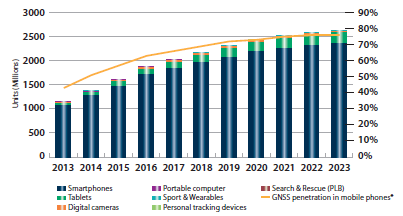
\includegraphics[scale=0.8]{./Figures/stats.png} \\
			\caption {Appareils GNSS par plate-forme. \cite{marketreport}}
		\end{figure}
\end{frame}
\begin{frame}
	\frametitle{Définition GNSS}
		\justifying
		\textbf{GNSS:} \textit{Global Navigation Satellite System} (Système de navigation par satellite global)\\
		Constellation de satellites permettant de localiser un point sur la Terre.
		\begin{figure}
			\centering
			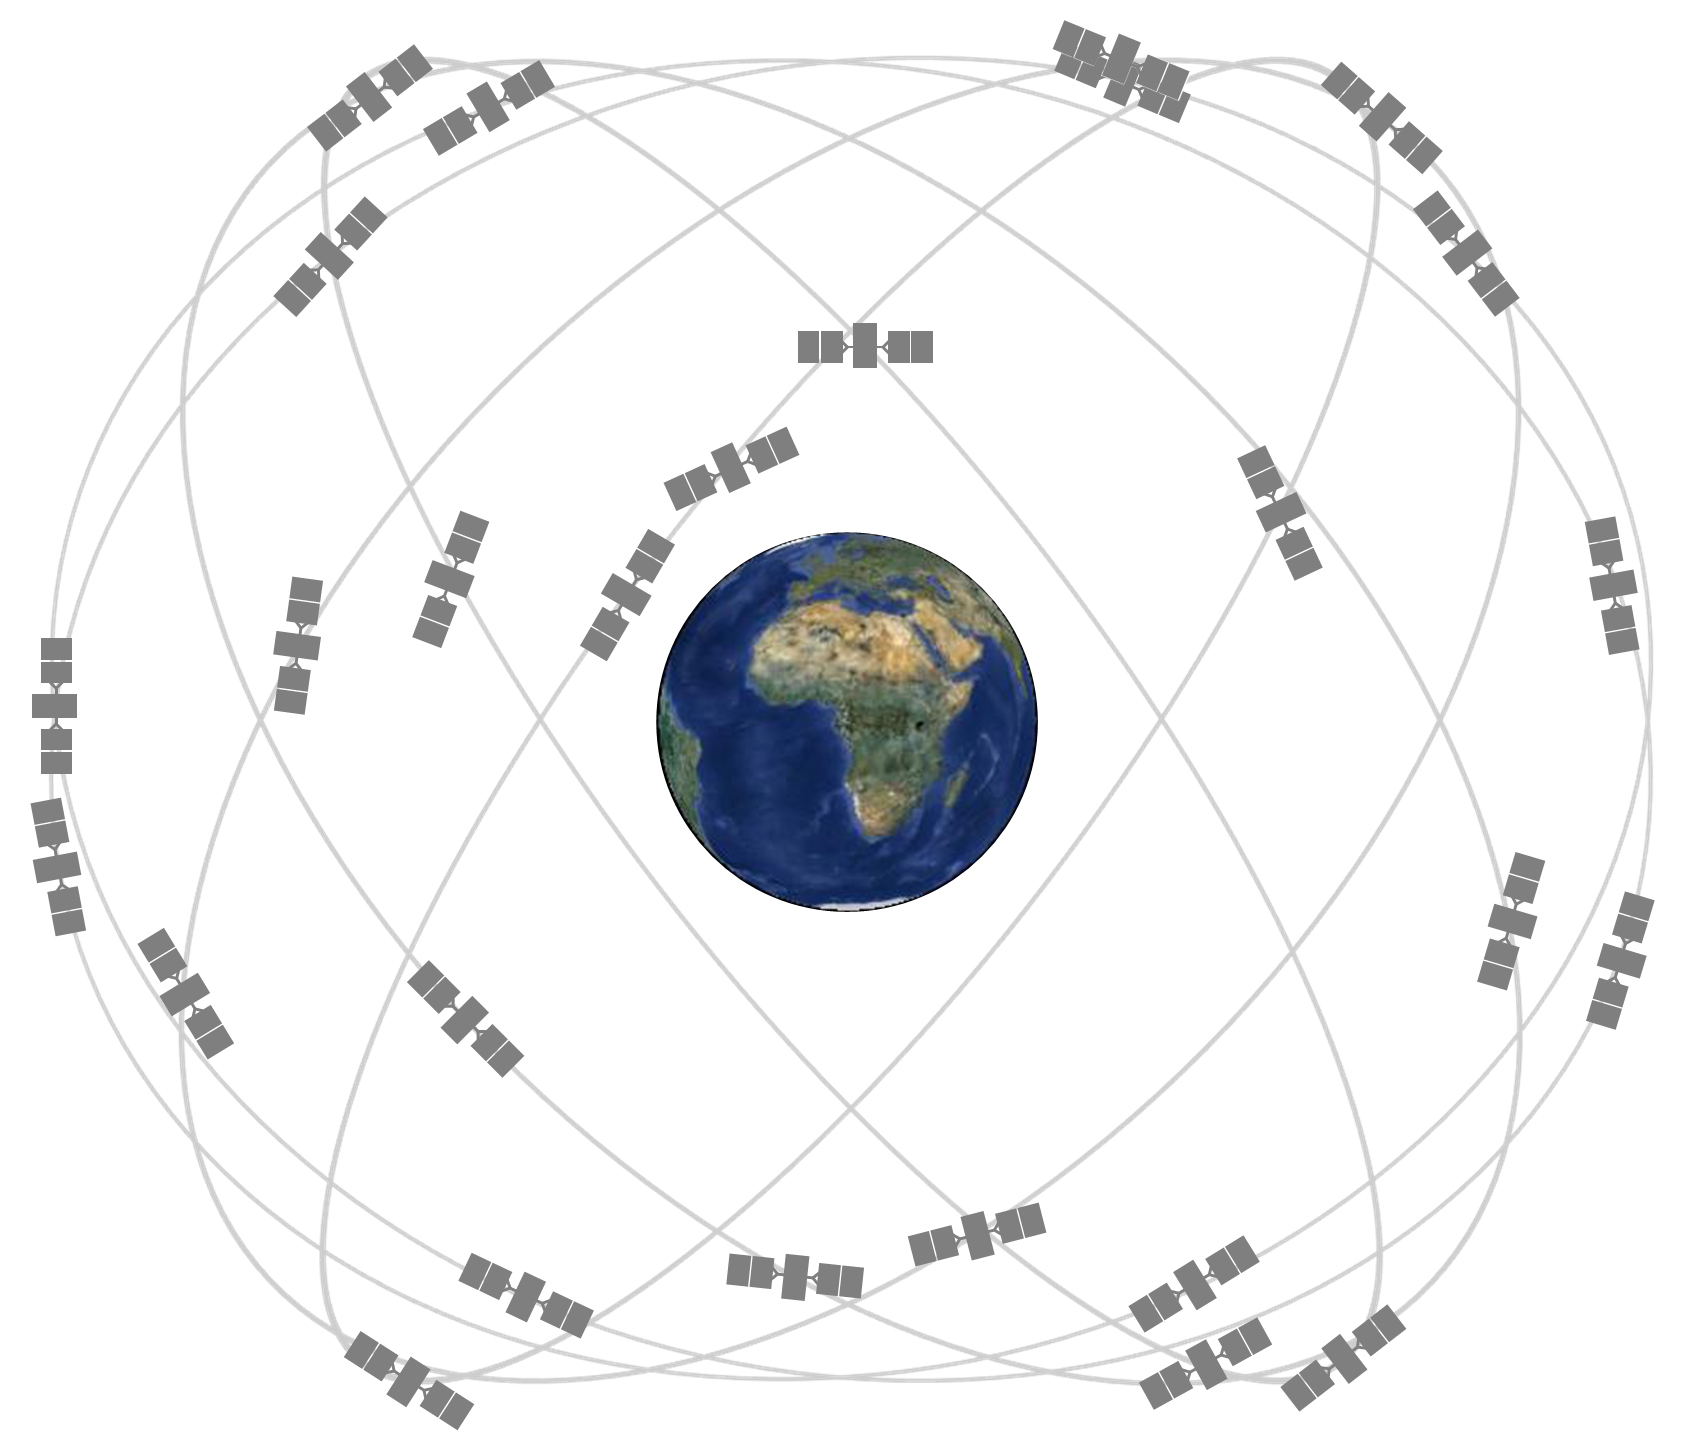
\includegraphics[width=0.3\textwidth]{./Figures/constellation.jpg} \\
			\caption {Système de navigation par satellite global. \cite{cons}}
		\end{figure}
\end{frame}

\begin{frame}
	\frametitle{Fonctionnement du GPS}
	\justifying
	\begin{columns}

		\begin{column}{0.5\textwidth}
			\begin{figure}
				\centering
				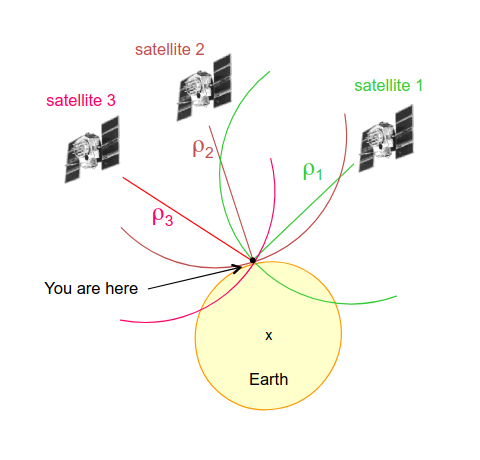
\includegraphics[width=0.9\textwidth]{./Figures/ENS_gnss.png} \\
				\caption {Fonctionnement du GPS. \cite{ens}}
			\end{figure}
		\end{column}

		\begin{column}{0.5\textwidth}
			Une sphère de rayon $\rho_1 = (\Delta t_1 \cdot c) $ \\
			3 satellites, intersection des 3 sphères.
			\newline
			Et donc {\footnotesize$\rho_s^s = \sqrt{(X^s-X_r)^2 + (Y^s-Y_r)^2 + (Z^s-Z_r)^2}$} \\
			Avec:
			\begin{itemize}
				\item $X^s, Y^s, Z^s$ : coordonnées du satellite $s$ ;
				\item $X_r, Y_r, Z_r$ : coordonnées du récepteur.
			\end{itemize}
		\end{column}

	\end{columns}

\end{frame}

\begin{frame}
	\frametitle{Sources d'incertitude}
	\justifying
	\begin{itemize}
		\item Les horloges des satellites et des récepteurs ne sont pas synchronisés. ($\delta t$)
		\item Réfraction lors de la propagation dans l’atmosphère :
		\item \begin{enumerate}
			\item Troposphérique (dépend de la température et de la pression atmosphérique) ($T_r^s$)
			\item Ionosphérique (dépend de la densité ionique) ($I_r^s$)
		\end{enumerate}
	\end{itemize}
	Modèle plus complet :
	\begin{equation}
		\boxed{R_r^s = \rho_r^s + c\delta t + T_r^s + I_r^s + ...}
	\end{equation}
\end{frame}
\begin{frame}
	\frametitle{Précision des orbites}
	\justifying
	Les systèmes GNSS sont basés sur des orbites prédites émises par les satellites. \\
	Ces \textbf{éphémérides} doivent donc être très précises. {\small(Perturbation gravitationnelle (cf. Annexe 1))} \\
	\begin{figure}
		\centering
		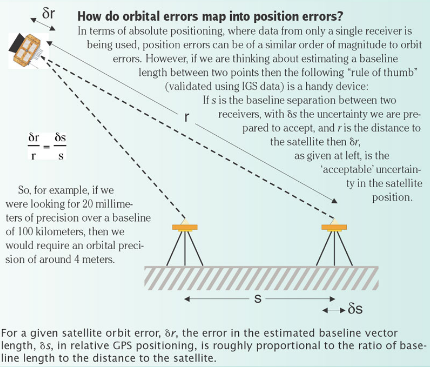
\includegraphics[width=0.35\textwidth]{./Figures/ENS_gnss2.png} \\
		\caption {Précision des orbites. \cite{ens}}
	\end{figure}
	{\small	\textit{Il existe aussi des services qui recalculent les éphémérides apostériori. (eg. IGN)}}
\end{frame}
\begin{frame}
	\frametitle{Multipath et dilution}
	\justifying
	\begin{columns}
		\begin{column}{0.5\textwidth}
			Le \textbf{multipath} (multi-trajet): le signal émis par le satellite est réfléchi par un objet avant d'atteindre le récepteur. (cf. Figure \ref{fig:multipath})
			\begin{figure}
				\centering
				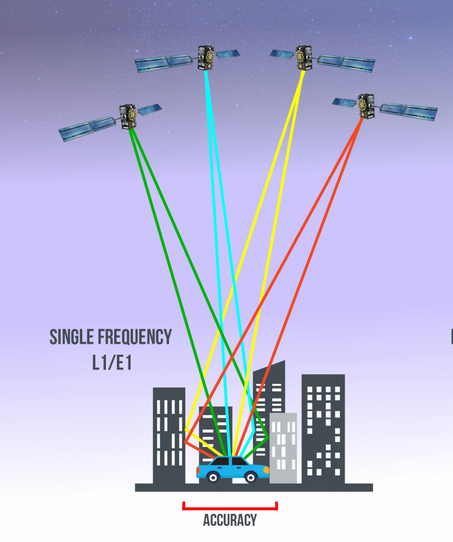
\includegraphics[width=0.5\textwidth]{./Figures/multipath.png} \\
				\caption {Multipath \cite{esa}}
				\label{fig:multipath}
			\end{figure}
		\end{column}
		\begin{column}{0.5\textwidth}
			La \textbf{dilution} (GDOP): la géométrie des satellites par rapport au récepteur influe sur la précision de la mesure. (cf. Figure \ref{fig:dilution})
			\begin{figure}
				\centering
				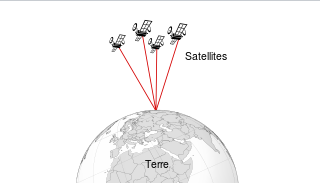
\includegraphics[width=0.8\textwidth]{./Figures/dilution.png} \\
				\caption {Coef. de dilution élevée \cite{esa}}
				\label{fig:dilution}
			\end{figure}
			
		\end{column}
	\end{columns}
\end{frame}

\begin{frame}{\frametitle{Sommaire}\tableofcontents}\end{frame}

\begin{frame}
	\frametitle{Problématique}
	\centering
	\begin{block}
		\scshape
			\begin{center}
				\Huge\emph{Comment peut-on réduire l'impact de l'urbanisation sur les systèmes GNSS pour améliorer la
				précision de la géolocalisation par satellite ?}
			\end{center}
	\end{block}
\end{frame}

\begin{frame}
	\frametitle{Objectifs}
	\justifying
	\begin{enumerate}
		
		\item Étude du GPS, fonctionnement rapide
		\item Impact de l'ionosphère et des corrections possibles
		\item Étude du multipath, dilution géométrique, GPS à doubles fréquences, et C/N0
		\item Comparaison Ville / campagne de la précision.
		\item Ouverture, solution possible (SBAS (systèmes d'optimisation de la précision par satellite), DGNSS (GNSS Différentiel), etc.)
	
	\end{enumerate}
\end{frame}
%---------- DEFINITION/PRELIMINARY ---------------------
\section{L'ionosphère}
\begin{frame}
	\frametitle{Définition}
	\begin{columns}
	    \justifying
		\begin{column}{0.5\textwidth}
	    	\textbf{L'ionosphère :} 
			L'ionosphère est la couche de l'atmosphère située entre 60 et 1000 km d'altitude.
			Elle est constituée de particules chargées électriquement, les ions, qui sont en mouvement.
		\end{column}
		\begin{column}{0.5\textwidth}
			\begin{figure}
				\centering
				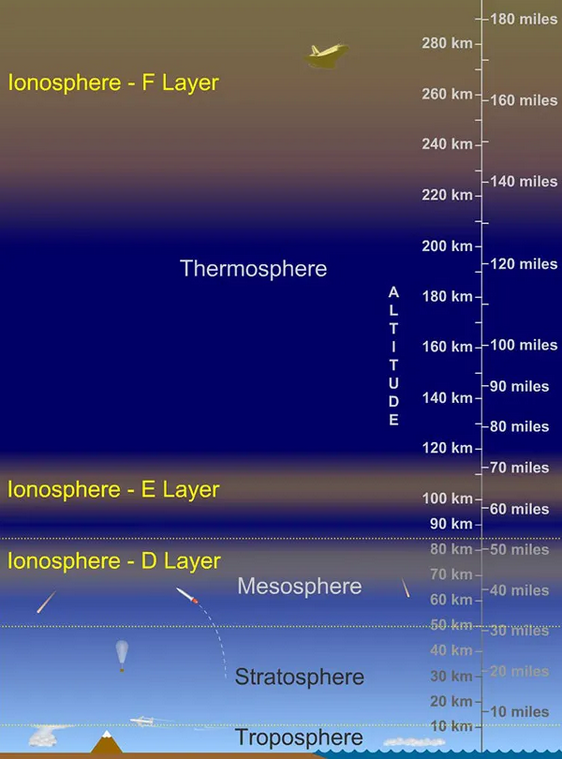
\includegraphics[width=0.7\textwidth]{./Figures/iono_ucar.png}
				\caption {Régions de l'ionosphère \cite{ucar}}	
			\end{figure}
		\end{column}	
	\end{columns}
\end{frame}
\begin{frame}
	\frametitle{Impact sur la propagation}
		\justifying
		\begin{columns}
			\begin{column}{0.5\textwidth}
				\textbf{Impact sur la propagation :} 
				\begin{itemize}
					\item \textbf{Propagation directe} - La propagation directe est la propagation d'une onde radio entre deux points sans interaction avec l'ionosphère.
					\item \textbf{Propagation diffusée} - La propagation diffusée est la propagation d'une onde radio entre deux points avec interaction avec l'ionosphère.
				\end{itemize}
			\end{column}
			\begin{column}{0.5\textwidth}
				\begin{figure}
					\centering
					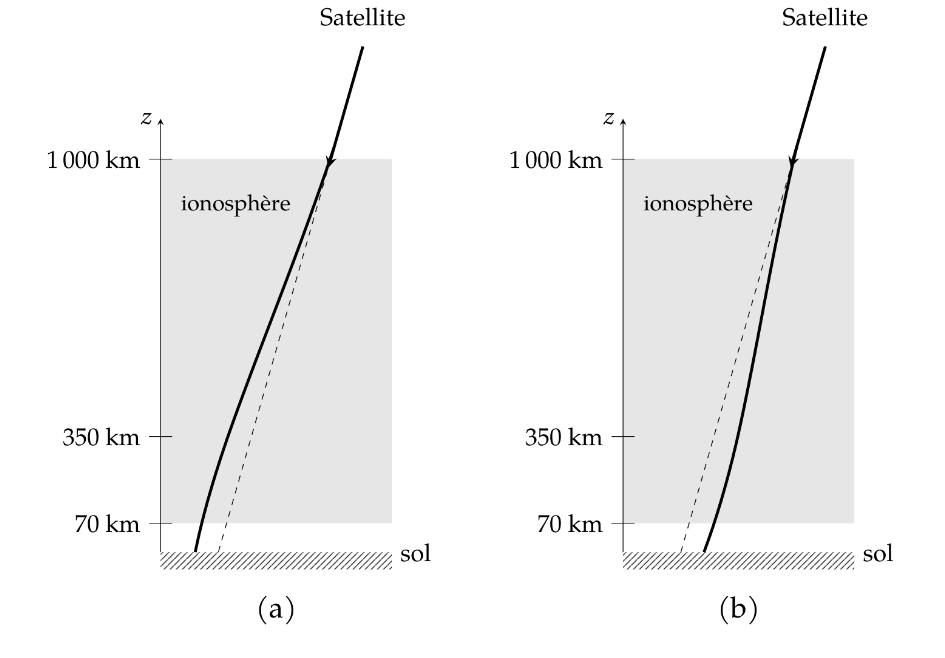
\includegraphics[width=0.7\textwidth]{./Figures/iono_e3a.png}
					\caption {Propagation directe et diffusée \cite{e3a}}	
				\end{figure}
			\end{column}
	\end{columns}
\end{frame}
\begin{frame}
	\frametitle{Quelle erreur ?}
	\justifying
		\begin{columns}
			\begin{column}{0.5\textwidth}
				\begin{figure}
					\centering
					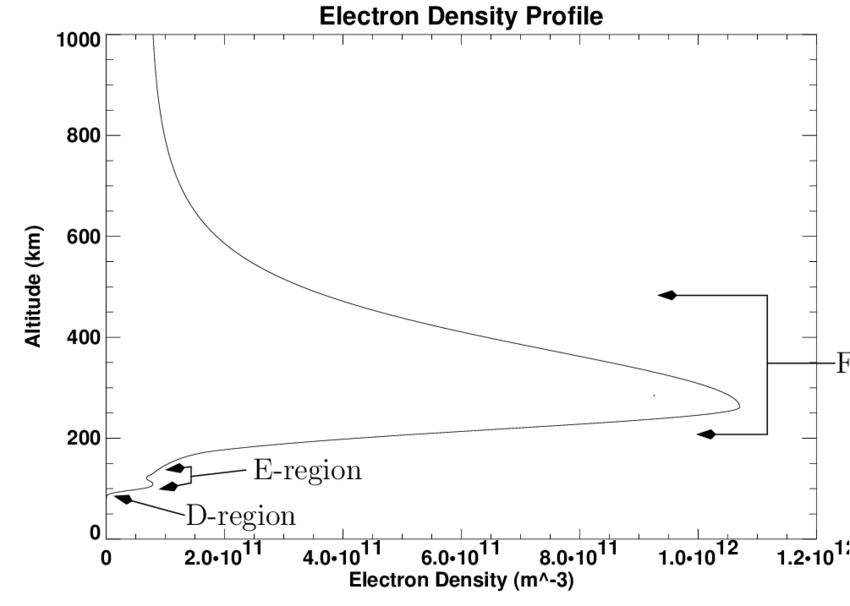
\includegraphics[width=1\textwidth]{./Figures/iono_profil.png}
					\caption {Profil Ionosphérique \cite{ionoprofil}}
				\end{figure}
			\end{column}
			\begin{column}{0.5\textwidth}

				Retard Ionosphérique : \\
				$\tau = \frac{1}{c} \int_{0}^{H_0} (\frac{c}{v_g}-1)$ \newline

				Erreur de distance : \\
				$L = \frac{a}{f_1^1} C_{ET}$ avec $C_{ET} = \int_{0}^{H_0} n_e dz$ (Contenu Électronique Total)
				\newline

				\begin{center}
					\textbf{A un TEC de }$1.5\cdot 10^{17} m^{-2}$, \boxed{$L = 220m$}
				\end{center}

				On a besoin de la \textbf{phase} et de la \textbf{speudorange} sur deux fréquences.
				\begin{flushright}
					\tiny{(Voir Annexe 2)}
				\end{flushright}
			\end{column}
		\end{columns}
\end{frame}

\begin{frame}{GPS à doubles fréquences}
	\justifying
	\textbf{Afin de calculer le TEC, un récepteur Dual-Band (L1, L5) est nécessaire :}
	\newline
	\begin{columns}
		\begin{column}{0.5\textwidth}
			\begin{figure}
				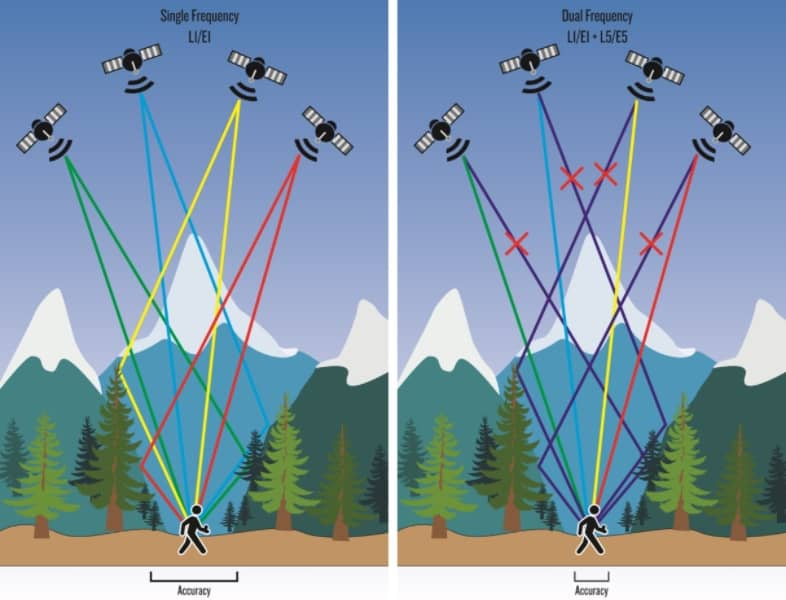
\includegraphics[width=0.9\textwidth]{./Figures/dual_band.jpg}
				\caption{\textit{Image: Garmin}}
			\end{figure}
		\end{column}
		\begin{column}{0.5\textwidth}
			Désormais disponible dans les smartphones(depuis 2018):
			\begin{figure}
				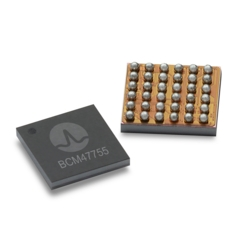
\includegraphics[width=0.7\textwidth]{./Figures/BCM47755.jpg}
				\caption{Broadcom BCM47755, \textit{Broadcom Inc.}}
			\end{figure}
		\end{column}
	\end{columns}
\end{frame}


%----------- MAIN RESULTS ------------------------------
\section{Expérimentations Ionosphérique}
\begin{frame}
	\centering
	\begin{block}
		\scshape
		\begin{center}
			\Huge Expérimentations Ionosphérique
		\end{center}
	\end{block}
\end{frame}
\begin{frame}{Préambule}
        \textbf{Méthode d'évaluation:} 
		Le CET \textit{Total electron content} s'évalue grâce à un même signal sur deux fréquences.

        \textbf{Le signal GPS:} 
	    \begin{itemize}
            \item \textbf{Speudorange} - La speudorange (distance) s'évalue à l'aide d'une fonction de corrélation.
            \item \textbf{Phase} - La phase s'évalue sur le nombre de phases depuis le début d'acquisition.
        \end{itemize}
		\begin{flushright}
			\tiny{(Voir Annexe 3)}
		\end{flushright}
\end{frame}

\begin{frame}{Protocole expérimental}
	RTKlib avec et sans correction ionosphérique.
	Calcul du TEC à partir de la phase et de la speudorange.
\end{frame}

\begin{frame}{Résultats}
	\begin{figure}
		\centering
		%\includegraphics[width=0.7\textwidth]{./Figures/tec.png}
		\caption {TEC en fonction du temps}	
	\end{figure}
\end{frame}

\section{Multipath}
\begin{frame}{Multipath}
	\begin{columns}
		\begin{column}{0.5\textwidth}
			\textbf{Multipath :} 
			Le multipath est un phénomène de propagation d'onde radio qui se propage sur plusieurs trajets entre l'émetteur et le récepteur.
			\newline
			Le multipath s'estime par : $MP = P - (\frac{2}{\alpha - 1} + 1) \cdot L_1 + \frac{2}{\alpha - 1} \cdot \L_2$
			\begin{flushright}
				\tiny{(Voir Démonstration Annexe 4)}
			\end{flushright}
			{\small \textbf{avec} $P$ la phase, $L_1$ la speudorange, $L_2$ la speudorange sur la deuxième fréquence et $\alpha$ le coefficient de réflexion.}
		\end{column}
		\begin{column}{0.5\textwidth}
			\begin{figure}
				\centering
				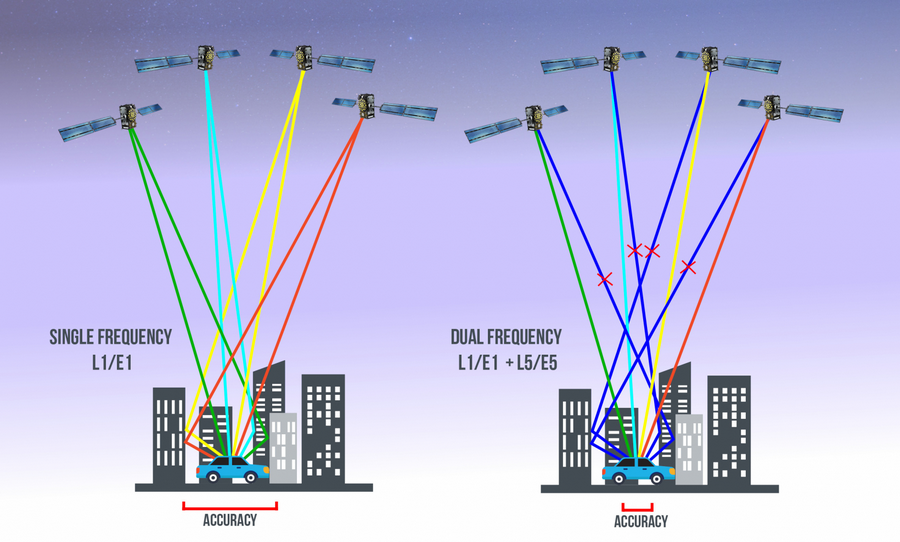
\includegraphics[width=0.9\textwidth]{./Figures/multipath2.png}
				\caption {Multipath \cite{esa}}	
			\end{figure}
			On a donc besoin de la \textbf{phase} et de la \textbf{speudorange} sur deux fréquences.
		\end{column}	
	\end{columns}
\end{frame}

\begin{frame}{Quelle erreur ?}
\begin{columns}
	\begin{column}{0.5\textwidth}
		\begin{figure}
			\centering
			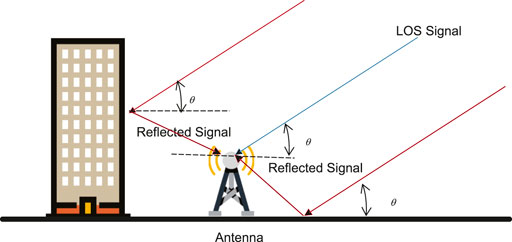
\includegraphics[width=0.8\textwidth]{./Figures/mp.jpg}
			\caption {Description du multipath \cite{10.3389/fphy.2022.1071539}}
		\end{figure}
		L'erreur est de \textbf{plusieurs mètres.} \cite{mperr}
	\end{column}
	\begin{column}{0.5\textwidth}
		\begin{figure}
			\centering
			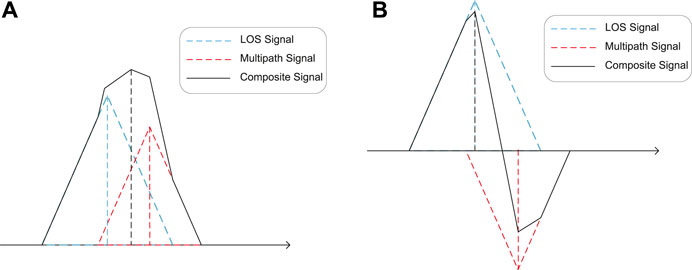
\includegraphics[width=0.7\textwidth]{./Figures/correl.jpg}
			\caption {Impact sur la fonction de corrélation {\tiny (\textit{Annexe 3})}}
		\end{figure}

		\begin{figure}
			\centering
			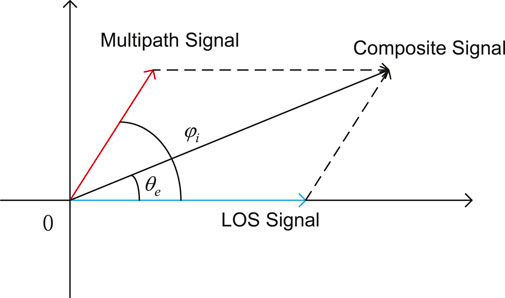
\includegraphics[width=0.7\textwidth]{./Figures/phase.jpg}
			\caption {Impact sur la phase}
		\end{figure}
	\end{column}
\end{columns}	
\end{frame}

\section{Expérimentations Multipath}
\begin{frame}
	\centering
	\begin{block}
		\scshape
		\begin{center}
			\Huge Expérimentations Multipath
		\end{center}
	\end{block}
\end{frame}

\begin{frame}{Protocole expérimental}
	\begin{itemize}
		\item Calcul du multipath à partir de la phase et de la speudorange.
		\item Basé sur un article de Umberto et al. \cite{mi8}
	\end{itemize}
\end{frame}

\begin{frame}{Résultats}
	\begin{figure}
		\centering
		%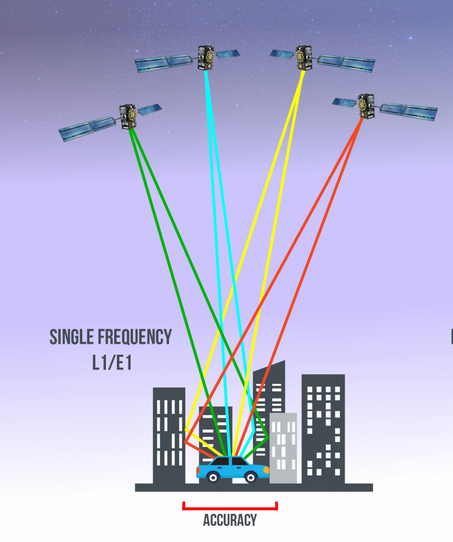
\includegraphics[width=0.7\textwidth]{./Figures/multipath.png}
		\caption {Multipath en fonction du temps}	
	\end{figure}
\end{frame}
\miniframesoff
\begin{frame}
	\centering
	\begin{block}
		\scshape
			\begin{center}
				\Huge\emph{Des Questions ?}
			\end{center}
	\end{block}
\end{frame}

\miniframeson
\appendix
\begin{frame}[allowframebreaks]
	\frametitle{Bibliographie}
	\printbibliography
\end{frame}

\section{Annexe 1}
\begin{frame}
	\label{appendix:1}
	\frametitle{Modélisation, perturbation gravitationnelle}
	
\end{frame}

\section{Annexe 2}
\begin{frame}
	\label{appendix:2}
	\frametitle{Démonstration TEC}

	\begin{columns}
		\begin{column}{0.5\textwidth}
			{\small Modélisation de l'onde par: $\vec{\underline{E}} = \vec{\underline{E_0}} \cdot exp(i(\omega t - kx))$ \\
			\textbf{Hypothèses :} \\ Poids et champ magnétique négligeable devant le champ électrique.\\ 
			\textbf{PDF et passage en complexe :} $m_e \frac{d \vec{\underline{v_e}}}{dt} = -e \vec{\underline{E}} \leftrightarrow i m_e \omega \vec{\underline{v_e}} = -e \vec{\underline{E}}$
			\\ Par définition : $\vec{\underline{j_e}}= -e n_e \vec{\underline{v_e}}$, soit: $\vec{\underline{j_e}} = \frac{e^2 n_e}{i m_e \omega} \vec{\underline{E}}$ \\
			D'après l'équation de propagation : $\vec{\Delta} \vec E - \frac{1}{c^2} \frac{\partial^2 \vec E}{\partial t^2} = \mu_0 \frac{\partial \vec j}{\partial t}$ \\
			On en déduit le signal complexe : $k^2 = \frac{\omega^2}{c^2} - \frac{e^2 n_e}{c^2 \epsilon_0 m_e}$ \\
			\textbf{Vitesse de phase :} $v_{\phi} = \frac{\omega}{k} = \frac{c}{\sqrt{1 - \frac{{f_p}^2}{f^2}}}$ \\
			
			}
			\end{column}

		\begin{column}{0.5\textwidth}
			\begin{flushright}
				L'indice est inférieur à 1, ... \\
				{\tiny \textit{D'après sujet E3A, \cite{e3a}}}
			\end{flushright}
		\end{column}
	\end{columns}
\end{frame}

\section{Annexe 3}
\begin{frame}
	\label{appendix:3}
	\frametitle{Le signal GPS}
	\begin{columns}
		\begin{column}{0.5\textwidth}
			Les récepteurs génèrent les fréquences porteuses L1 et L5 et compare avec celui reçu :
			\begin{figure}
				\centering
				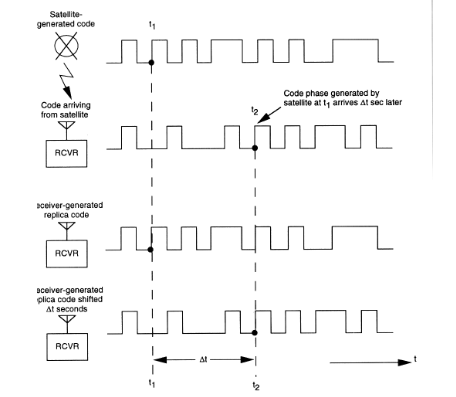
\includegraphics[width=0.8\textwidth]{./Figures/correl1.png}
				\caption {Décodage \cite{ens}}
			\end{figure}
		\end{column}
		\begin{column}{0.5\textwidth}
			Détermine le pic de corrélation (code GOLD) et en déduit le décalage temporel.
			\begin{figure}
				\centering
				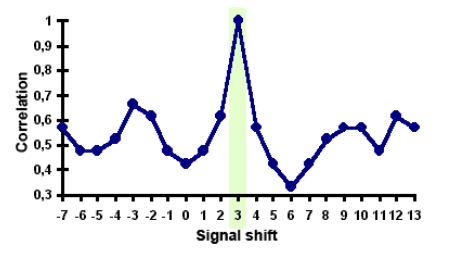
\includegraphics[width=0.8\textwidth]{./Figures/correl2.png}
				\caption {Fonction de corrélation \cite{ens}}
			\end{figure}
		\end{column}
	\end{columns}
\end{frame}

\section{Annexe 4}
\begin{frame}
	\label{appendix:4}
	\frametitle{Démonstration Multipath}

	\begin{columns}
		\begin{column}{0.5\textwidth}
			{\small
			On \textbf{modélise les signaux} $L_1$ et $L_5$ par: \\
			$P_1 = R +I1 +MP1$ et $P_5 = R + I5 + MP5$ \\
			\textit{Avec : $R$ la distance réelle, $I1$ et $I5$ les erreurs ionosphériques, $MP1$ et $MP5$ les erreurs multipath.} \\
			Ainsi que leurs \textbf{phases respectives :} \\
			$L_1 = R - I1 + mp1 + B1$ et $L_5 = R - I5 + mp5 + B5$ \\
			\textit{Avec : $B1$ et $B5$ les ambiguïtés de phase. On néglige $mp << MP \leftrightarrow mp=0$} \\
			D'après \textit{Annexe 3} $I_i = \frac{A}{f_i^2}T_{EC}$ soit: 
			\begin{center}
				$\frac{I_5}{I_2} = \frac{f_1}{f_5}^2 = \alpha$
			\end{center}
			}
		\end{column}

		\begin{column}{0.5\textwidth}
			Après calcul des différentes combinaisons, \textbf{on obtient :} \\
			{\small $MP1 - P1 + (\frac{2}{\alpha - 1} + 1)L1 - (\frac{2}{\alpha - 1}) L5 = cte$} \\
			Comme le multipath est à valeur moyenne nulle, \textbf{on a :} \newline

			{\footnotesize \boxed{MP1 = P1 - (\frac{2}{\alpha - 1} + 1)L1 + (\frac{2}{\alpha - 1}) L5}} \newline

			\textbf{De même pour $MP5$ :} \newline
			
			{\footnotesize \boxed{MP5 = P5 - (\frac{2 \alpha}{\alpha - 1})L1 + (\frac{2 \alpha}{\alpha - 1} - 1)L5}} \\

			\begin{flushright}
				{\tiny \textit{D'après Eric Calais, \cite{ens}}}
			\end{flushright}
		\end{column}
	\end{columns}
\end{frame}
%--------- THANK YOU Text ------- texlive-most -------------------
%----------------------------------------------------
\end{document}
